% This is "sig-alternate.tex" V2.0 May 2012
% This file should be compiled with V2.5 of "sig-alternate.cls" May 2012
%
% This example file demonstrates the use of the 'sig-alternate.cls'
% V2.5 LaTeX2e document class file. It is for those submitting
% articles to ACM Conference Proceedings WHO DO NOT WISH TO
% STRICTLY ADHERE TO THE SIGS (PUBS-BOARD-ENDORSED) STYLE.
% The 'sig-alternate.cls' file will produce a similar-looking,
% albeit, 'tighter' paper resulting in, invariably, fewer pages.
%
% ----------------------------------------------------------------------------------------------------------------
% This .tex file (and associated .cls V2.5) produces:
%       1) The Permission Statement
%       2) The Conference (location) Info information
%       3) The Copyright Line with ACM data
%       4) NO page numbers
%
% as against the acm_proc_article-sp.cls file which
% DOES NOT produce 1) thru' 3) above.
%
% Using 'sig-alternate.cls' you have control, however, from within
% the source .tex file, over both the CopyrightYear
% (defaulted to 200X) and the ACM Copyright Data
% (defaulted to X-XXXXX-XX-X/XX/XX).
% e.g.
% \CopyrightYear{2007} will cause 2007 to appear in the copyright line.
% \crdata{0-12345-67-8/90/12} will cause 0-12345-67-8/90/12 to appear in the copyright line.
%
% ---------------------------------------------------------------------------------------------------------------
% This .tex source is an example which *does* use
% the .bib file (from which the .bbl file % is produced).
% REMEMBER HOWEVER: After having produced the .bbl file,
% and prior to final submission, you *NEED* to 'insert'
% your .bbl file into your source .tex file so as to provide
% ONE 'self-contained' source file.
%
% ================= IF YOU HAVE QUESTIONS =======================
% Questions regarding the SIGS styles, SIGS policies and
% procedures, Conferences etc. should be sent to
% Adrienne Griscti (griscti@acm.org)
%
% Technical questions _only_ to
% Gerald Murray (murray@hq.acm.org)
% ===============================================================
%
% For tracking purposes - this is V2.0 - May 2012

\documentclass{sig-alternate}

\usepackage{listings}
\usepackage[usenames,dvipsnames]{color}
\usepackage{multirow}
\usepackage{array}
%\usepackage{natbib}% bold math
\newcommand{\ddx}[2]{ \frac{ \partial #1}{ \partial {#2} } }
%\newcommand{\ddt}[1]{ \frac{\partial #1}{\partial t} }
\newcommand{\ddt}[1]{\partial_t #1}
\newcommand{\Grad}[1]{\nabla #1}
\newcommand{\Div}[1]{\Grad \cdot #1}
\newcommand{\Lap}[1]{\Delta #1}
\definecolor{light-gray}{gray}{0.95}

\lstdefinestyle{cxx}{ %
language=C++,
basicstyle=\footnotesize\ttfamily,  % the size of the fonts that are used for the code
% numbers=left,                   % where to put the line-numbers
% numberstyle=\footnotesize,      % the size of the fonts that are used for the line-numbers
% stepnumber=2,                   % the step between two line-numbers. If it's 1 each line will be numbered
% numbersep=5pt,                  % how far the line-numbers are from the code
% backgroundcolor=\color{white},  % choose the background color. You must add \usepackage{color}
backgroundcolor=\color{light-gray},  % choose the background color. You must add \usepackage{color}
showspaces=false,               % show spaces adding particular underscores
commentstyle=\color{cyan},
stringstyle=\ttfamily\color{red},
showstringspaces=false,         % underline spaces within strings
showtabs=false,                 % show tabs within strings adding particular underscores
frame=single,                 % adds a frame around the code
tabsize=2,                      % sets default tabsize to 2 spaces
captionpos=b,                   % sets the caption-position to bottom
breaklines=true,                % sets automatic line breaking
breakatwhitespace=false,        % sets if automatic breaks should only happen at whitespace
title=\lstname,                 % show the filename of files included with \lstinputlisting; also try caption instead of title
% morekeywords={char,double},
escapeinside={\%*}{*)},          % if you want to add a comment within your code
% morekeywords={*,...}          % if you want to add more keywords to the set
% morekeywords={char,double}    % if you want to add more keywords to the set
frameround=fttt
}

\lstdefinestyle{fortran}{ %
language=Fortran,
basicstyle=\footnotesize\ttfamily,  % the size of the fonts that are used for the code
% numbers=left,                   % where to put the line-numbers
% numberstyle=\footnotesize,      % the size of the fonts that are used for the line-numbers
% stepnumber=2,                   % the step between two line-numbers. If it's 1 each line will be numbered
% numbersep=5pt,                  % how far the line-numbers are from the code
% backgroundcolor=\color{white},  % choose the background color. You must add \usepackage{color}
backgroundcolor=\color{light-gray},  % choose the background color. You must add \usepackage{color}
showspaces=false,               % show spaces adding particular underscores
commentstyle=\color{cyan},
stringstyle=\ttfamily\color{red},
showstringspaces=false,         % underline spaces within strings
showtabs=false,                 % show tabs within strings adding particular underscores
frame=single,                 % adds a frame around the code
tabsize=2,                      % sets default tabsize to 2 spaces
captionpos=b,                   % sets the caption-position to bottom
breaklines=true,                % sets automatic line breaking
breakatwhitespace=false,        % sets if automatic breaks should only happen at whitespace
title=\lstname,                 % show the filename of files included with \lstinputlisting; also try caption instead of title
% morekeywords={char,double},
escapeinside={\%*}{*)},          % if you want to add a comment within your code
% morekeywords={*,...}          % if you want to add more keywords to the set
% morekeywords={char,double}    % if you want to add more keywords to the set
frameround=fttt
}

\newcommand{\kk}[1]{{\color{blue}{\it KK: #1}}}

\begin{document}

%% \title{A Sample {\ttlit ACM} SIG Proceedings Paper in LaTeX
%% Format\titlenote{(Does NOT produce the permission block, copyright information nor page numbering). For use with ACM\_PROC\_ARTICLE-SP.CLS. Supported by ACM.}}
%% \subtitle{[Extended Abstract]
%% \titlenote{A full version of this paper is available as
%% \textit{Author's Guide to Preparing ACM SIG Proceedings Using
%% \LaTeX$2_\epsilon$\ and BibTeX} at
%% \texttt{www.acm.org/eaddress.htm}}}

%\conferenceinfo{EuroMPI}{2013 Madrid, Spain}

\title{
Efficient evaluation of threshold queries of derived fields in a numerical simulation database
}
%
% You need the command \numberofauthors to handle the 'placement
% and alignment' of the authors beneath the title.
%
% For aesthetic reasons, we recommend 'three authors at a time'
% i.e. three 'name/affiliation blocks' be placed beneath the title.
%
% NOTE: You are NOT restricted in how many 'rows' of
% "name/affiliations" may appear. We just ask that you restrict
% the number of 'columns' to three.
%
% Because of the available 'opening page real-estate'
% we ask you to refrain from putting more than six authors
% (two rows with three columns) beneath the article title.
% More than six makes the first-page appear very cluttered indeed.
%
% Use the \alignauthor commands to handle the names
% and affiliations for an 'aesthetic maximum' of six authors.
% Add names, affiliations, addresses for
% the seventh etc. author(s) as the argument for the
% \additionalauthors command.
% These 'additional authors' will be output/set for you
% without further effort on your part as the last section in
% the body of your article BEFORE References or any Appendices.

\numberofauthors{3} %  in this sample file, there are a *total*
% of EIGHT authors. SIX appear on the 'first-page' (for formatting
% reasons) and the remaining two appear in the \additionalauthors section.
%
\author{
% You can go ahead and credit any number of authors here,
% e.g. one 'row of three' or two rows (consisting of one row of three
% and a second row of one, two or three).
%
% The command \alignauthor (no curly braces needed) should
% precede each author name, affiliation/snail-mail address and
% e-mail address. Additionally, tag each line of
% affiliation/address with \affaddr, and tag the
% e-mail address with \email.
\alignauthor Kalin Kanov \\
     \affaddr{Department of Computer Science} \\
     \affaddr{IDIES} \\
     \affaddr{Johns Hopkins University} \\
     \affaddr{Baltimore, MD 21218} \\
     \email{kalin@cs.jhu.edu}
\alignauthor Randal Burns \\
     \affaddr{Department of Computer Science} \\
     \affaddr{IDIES} \\
     \affaddr{Johns Hopkins University}\\
     \affaddr{Baltimore, MD 21218} \\
     \email{randal@cs.jhu.edu} 
\alignauthor Cristian C. Lalescu \\
     \affaddr{Department of Applied Mathematics and Statistics} \\
     \affaddr{IDIES} \\
     \affaddr{Johns Hopkins University} \\
     \affaddr{Baltimore, MD 21218} \\
     \email{clalesc1@jhu.edu}
}
%% \and % use '\and' if you need 'another row' of author names
%% % There's nothing stopping you putting the seventh, eighth, etc.
%% % author on the opening page (as the 'third row') but we ask,
%% % for aesthetic reasons that you place these 'additional authors'
%% % in the \additional authors block, viz.
%% \additionalauthors{Additional authors: John Smith (The Th{\o}rv{\"a}ld Group,
%% email: {\texttt{jsmith@affiliation.org}}) and Julius P.~Kumquat
%% (The Kumquat Consortium, email: {\texttt{jpkumquat@consortium.net}}).}
%% \date{30 July 1999}
%% % Just remember to make sure that the TOTAL number of authors
%% % is the number that will appear on the first page PLUS the
%% % number that will appear in the \additionalauthors section.

\maketitle

\begin{abstract}
Large numerical simulations are commonplace in the study of many different physical phenomena. 
The datasets produced by these simulations are in the TB and
even PB ranges. Data-intensive architectures and compute clusters have been deployed to store, manage and provide public access to such datasets. 
The systems built on top of these architectures, sometimes called virtual laboratories, usually do not support the analysis functionality that scientists are 
interested in out of the box. Moreover, data-intensive computations that examine entire time-steps of the simulation data are impractical to perform
locally and can take days or months to iterate over the entire dataset. 
In this paper we present a method for the efficient evaluation of threshold queries of derived fields for large numerical 
simulation datasets
stored in a cluster of relational databases. The method achieves scalability through data-parallel execution. We introduce an application-aware 
cache for query results, which has little overhead and improves query performance by over an order of magnitude for queries that hit the cache.

\end{abstract}

%% % A category with the (minimum) three required fields
%\category{}{Extending Data Base Technology}
%% %A category including the fourth, optional field follows...
%% \category{D.2.8}{Software Engineering}{Metrics}[complexity measures, performance measures]

%\terms{Extending Database Technology}

\keywords{databases, data-intensive computing, threshold queries, turbulence} % NOT required for Proceedings

\section{Introduction}
%What is the problem?
Better instruments, faster and bigger supercomputers and easier collaboration and sharing of data in the sciences have introduced the need
to manage increasingly large data sets. Data-intensive systems and architectures have been developed with the goal of storing and providing
fast access to such data sets. Examples include the GrayWulf and DataScope clusters \cite{Szalay, TODO} at Johns Hopkins, which have capacity 
of 1.1PB and xPB
respectively. They have been developed with the goal of providing persistent storage and public access to world-class numerical simulation data. 
These systems differ from the traditional HPC systems in that they aim to achieve high aggregate throughput by balancing computation
capabilities with I/O and network bandwidth. The computing systems and services developed on top of these platforms are more than pure
storage engines and usually have complex analysis routines built-in, which has largely been driven by the ``move the computation to the data"
paradigm. These built-in analysis routines are most often not novel themselves. They implement core scientific functionality for the study of the
particular scientific phenomena, which was observed or simulated in the first place. The analysis routines however require novel evaluation strategies 
and methods for their execution. They have to operate on large datasets distributed across multiple nodes of a cluster of relational databases 
and in order to reduce their running times they have to make efficient use of the cluster resources. 

Finding the locations or regions of highest vorticity or those with the largest norms of the velocity or other fields of interest is
functionality that enables new insights in the study of fluid dynamics. Furthermore, threshold, top-$k$ queries and similarity search in general
are important in many different disciplines. In this paper we introduce an efficient evaluation strategy for threshold
queries over time series datasets stored in a cluster of relational databases. Our method evaluates not only threshold queries of the vector or 
scalar field data stored in the database, but also performs thresholding of derived fields.

%Why is it hard? (E.g., why do naive approaches fail?)
The evaluation of threshold queries of derived fields requires a kernel computation at each point on the grid in order to compute the field to be thresholded.
The value of the derived field at each location depends on all the values at locations within the kernel of computation. 
In order to evaluate such a query for a given time-step all of the data for that time-step must be read and each data point 
will appear in $N$ kernels of computation, where $N$ is the size of the kernel. The evaluation is thus both data and computation intensive.
Obtaining the derived field and thresholding locally requires not only the computation of the derived field over an entire time-step but also the transfer of
a large amount of data most of which are subsequently discarded. 
It is also impractical to materialize all possible derived fields with the raw data
due to the large size of the datasets and the limits of available storage. Therefore, the derived fields 
have to be evaluated on-demand from the stored data and thresholding performed on the database nodes near the data.

Database, operating and file system caches are effective at speeding up access to the large amounts of data stored on disk. However, as was
shown by Lopez et al. \cite{Lopez} this might not be sufficient for some interactive applications. Moreover, even if the data are available in the cache the
computation associated with the derived field still needs to be performed for each point on the grid as results of previous computations are not cached. 

%Why is it interesting and important?
Thresholding allows scientists to obtain and examine the most intense regions and features in the dataset in the case of turbulence. 
These are often the locations that have the largest vorticity norms and have intense vortices or reconnection events. 
It is important that threshold queries are evaluated in an efficient manner, because often further subsequent examination
and analysis is required to understand the physics that drive these intense events. 

%Why hasn't it been solved before? (Or, what's wrong with previous proposed solutions? How does mine differ?)
Data-intensive architectures and compute clusters built from commodity hardware rely on parallel I/O to multiple disks and high network bandwidth
to achieve high throughput. Such systems have only recently been deployed for the storage of large numerical simulation 
datasets. The virtual laboratories built on these systems often do not support
all of the functionality that scientists are interested in. Database systems support rollup queries, including top-$k$ queries, but in most cases these
queries apply only simple linear score functions on the attribute values of individual records. 
We present a method for the efficient evaluation of threshold queries over fields derived from the raw vector or scalar fields of the numerical simulation 
stored in the database. The derived fields, which our method computes and operates on are derived by performing kernel computations over the array data 
stored in the database.
Our method makes effective use of the cluster resources and achieves high throughput and scalability. 

%What are the key components of my approach and results? Also include any specific limitations.
We exploit the parallelism 
available in the cluster by means of data-parallel execution of the computations. Each computation is distributed across the nodes of the cluster and
is executed in parallel by several threads within a database node by means of creating multiple connections to each node. Moreover we introduce an 
application-aware cache for query results. We build on the idea of an application-aware cache introduced by Lopez et al. \cite{Lopez} and more broadly 
on the concept of semantic caching \cite{Ren}. Rather than caching just data as is the case in system caches and the tree-cache described by Lopez et al.
we cache the actual results of the computation, which leads to query performance improvement of over an order of magnitude.

%-The evaluation is computationally limited and embarrassingly parallel, which makes it a good candidate for a GPU implementation.

\section{Scientific Use Cases}\label{science_use_cases}

\begin{figure}
\centering
\includegraphics[width=3.35in]{Figures/PDF.pdf}
\caption{Probability density function of the norm of the vorticity field for a representative time-step for the MHD dataset.}
\label{fig:pdf}
\end{figure}

%Max vorticity clustering.
One of the applications of thresholding in turbulence is to find the locations of maximum vorticity in a particular time-step or the dataset as a whole.
The locations of maximum vorticity are usually associated with the most intense vortices in the dataset and often have interesting and complex
reconnection events associated with them. 
Once obtained from the service, these locations can be clustered in both 3d and 4d. This allows scientists to examine their evolution with the flow
and make subsequent analysis queries as needed in order to study these events.

The vorticity is computed from the velocity field by taking its curl:
\begin{align}
\vec{\omega} &= \vec{\nabla} \times \vec{v} = \left( \frac{\partial}{\partial x}, \frac{\partial}{\partial y}, \frac{\partial}{\partial z} \right) 
\times \nonumber \left( v_x, v_y, v_z \right)\\
&= \left( \frac{\partial v_z}{\partial y} - \frac{\partial v_y}{\partial z}, \frac{\partial v_x}{\partial z} - \frac{\partial v_z}{\partial x}, 
\frac{\partial v_y}{\partial x} - \frac{\partial v_x}{\partial y} \right).
\label{eq:curl}
\end{align}
We use finite differencing methods of
different orders for the evaluation of the curl. For example, with 4th-order centered finite differencing each partial derivative is evaluated from the 4
adjacent grid node values as follows:  
\begin{align} 
\left.\frac{df}{dx}\right|_{x_n} = &\frac{2}{3\Delta x}[f(x_{n+1})-f(x_{n-1})]\nonumber\\ 
&-\frac{1}{12\Delta x}[f(x_{n+2})-f(x_{n-2})],
\end{align}
where $f$ denotes any one of the three components of the velocity and $\Delta x$ is the width of the grid in the $x$ direction. The partial derivatives
along $y$ and $z$ are computed in the same fashion. 
Fig. \ref{fig:pdf} shows the distribution of the values of the norm of the vorticity field in the MHD dataset for a representative time-step. This is indicative 
of how the values are distributed in the dataset as a whole.
This coarse view of the data can be used by scientists to guide the selection of threshold values.

- 3d and 4d clusters of highest vorticity locations. 

Similar to the vorticity there are other fields of interest, which can be thresholded. These include ...

\section{JHTDB}

\begin{figure*}
\centering
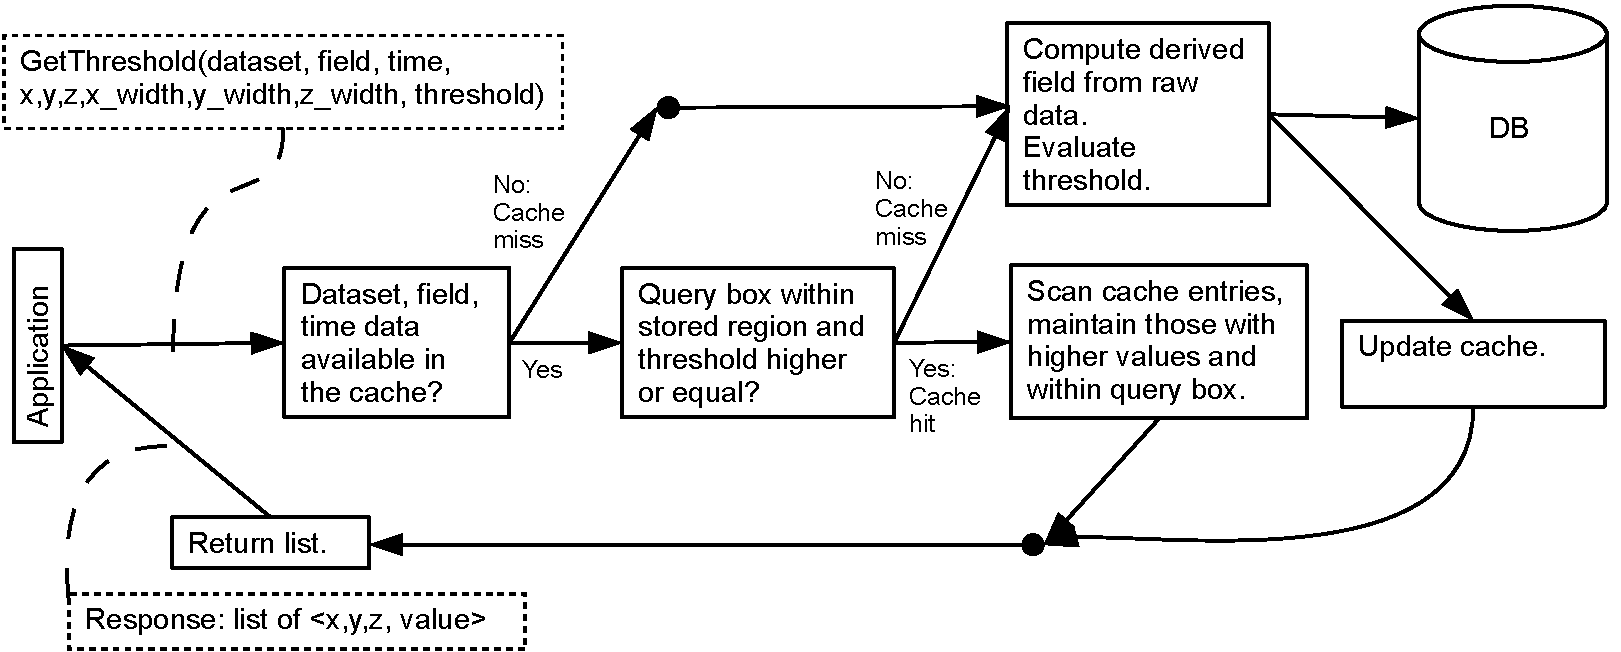
\includegraphics[width=6.5in]{Figures/cache_diagram.pdf}
\caption{Cache lookup.}
\label{fig:cache_diagram}
\end{figure*}

The method that we have developed for the evaluation of threshold queries of derived fields was deployed and integrated into the 
Johns Hopkins Turbulence Databases (JHTDB). The JHTDB, built on top of the GrayWulf and DataScope clusters, serve as a public virtual laboratory for
the study of turbulent phenomena. The JHTDB store several datasets, which are the output of high-resolution numerical simulations of turbulence.
The 3d time-series data are partitioned into small sub-cubes and stored in relational databases distributed across the nodes of the cluster.
Access to the data is provided by means of Web-services and a variety of analysis functions have been
implemented and can be executed through Web-service calls.
At present the service hosts four datasets, which are available publicly. 
The data are the output of numerical simulations of forced isotropic turbulence, magnetohydrodynamics (MHD), channel 
flow turbulence and homogenous buoyancy driven turbulence.
The total amount of space occupied by the datasets is over 230 TB. 

The database nodes are part of the GrayWulf \cite{Szalay} and DataScope \cite{TODO} clusters. Each node
is running Windows Server 2008 and SQL Server 2008 R2. The data for each dataset are partitioned spatially across 4 to 8
database nodes, and each database node hosts one or more databases. We use the Morton z-order space-filling
curve to distribute the data across nodes and databases as well as to spatially subdivide each time-step
into database atoms, which are of size $8^3$. Each such atom is indexed by the time-step, which it belongs to and
by the Morton code of it's lower left corner. This combination of index and data forms a record in the database.
Queries to the data and derived fields, such as derivatives and filtered quantities are evaluated through
stored procedures or user-defined functions implemented in the Common Language Runtime (CLR) framework.

The Web-services are hosted on a front-end Web-server, which handles user requests and hosts the main Web-page portal.
The Web-server acts as a mediator sending the users' requests to the database nodes and initiating their distributed evaluation. 
It assembles the results and sends them back to the client

The JHTDB provide a variety of data-intensive analysis routines that are executed on the database nodes. These include interpolation, 
differentiation, particle tracking and spatial filtering. These tasks are often data-intensive and in order to leverage the capabilities of the cluster we
have developed data-driven batch processing techniques for their evaluation \cite{KanovSC11, KanovSC12}. What differentiates threshold and
top-$k$ queries from these tasks is the fact that they usually operate on small subsets of the space or a collection of individual target locations, whereas
threshold and top-$k$ queries usually have to examine the entire data volume. Furthermore, the data product of threshold and top-$k$ queries is much
smaller in relation to the amount of data that need to be examined. This fact combined with the fact that subsequent queries can reuse previously
computed results makes the query results suitable to caching. 

\section{Threshold Query Evaluation}

Threshold queries of derived fields submitted to the JHTDB are evaluated using a data-parallel execution strategy and the query results are 
cached in an application-aware cache. The evaluation strategy for queries that do not hit the cache is driven by the spatial partitioning of the 
data across the nodes of the cluster.

{\bf Derived fields computation}. The databases store only the raw field data from the simulation (e.g. velocity, pressure, etc.). However, the threshold
queries that are of biggest interest to science users aim to obtain all locations where the values of a derived field are above a given threshold. Thus, the
derived field in question has to be computed from the raw data first. For most derived fields of interest this computation has local support. It has an 
associated localized kernel of computation around each grid node. Therefore, the value of the derived field at each grid node depends on the value of the
stored field at the grid locations, which are part of the kernel of computation. 

{\bf Distributed data-parallel execution}. In most cases threshold queries operate over an entire time-step. Each such query is subdivided by 
the mediator into queries submitted to
each of the database nodes. Each node evaluates the query over the data that it has stored locally. Only a small amount of data along the boundary
need to be requested from adjacent nodes. The data are read into memory and the particular field requested is computed at each of the locations on
the grid. The same strategy applies when utilizing multiple threads per node. The norm or absolute value of the derived field at each location is compared 
against the specified threshold and if the value is higher it is maintained along with
the spatial coordinates of the location in a list. We limit the maximum size of this list to around 1,000,000 locations in order to prevent having to return
the entire time-step or a significant fraction of it for queries with thresholds that are set too low. 

{\bf Application-aware cache for query results}. The central part of the evaluation strategy for threshold queries that we have developed is the 
introduction of an application-aware cache
for query results. The results of these queries are small compared to the amount of data that need to be examined and the results can be used to
answer subsequent queries as long as they are within the same region and specify the same or higher threshold. Each database node has a local 
cache. Cache entries are indexed by the field, time-step, spatial region and the threshold requested. We use a least recently
used cache replacement policy. All modifications of and queries to the cache are executed within a transaction with snapshot isolation level to
avoid dirty-reads or inconsistent view of the cache. Caching the query results
preserves the computational effort in addition to substantially reducing I/O. We do not have to derive the requested field from the raw data for 
queries that hit the cache. This results in a substantial improvement in query performance as we only have to scan
a small set of data and do not need to perform any additional computation.

%\kk{Cite results for top-$k$ queries in databases and distributed systems. Remark that non of these strategies operate on large array datasets 
%and they do not operate on derived fields, where each value of the derived field depends on multiple values from the original field and requires a kernel
%computation accessing multiple data points in a kernel around the target location.}

The cached query results are stored in a table in the database and the overall size of the cache is limited by the amount of available disk space, not memory.
The space required to cache the maximum number of points per time-step including the index space and database overhead is $\sim$40MB. 
Therefore for a dataset containing 
1024 time-steps, as is the case for the isotropic turbulence and MHD datasets part of the JHTDB, a cache size of 40GB is sufficient to cache the query
results for threshold queries of a derived field over the entire dataset. In contrast, computing and materializing a derived field for the entire dataset will
require $\sim$5TB.

\begin{figure}
\centering
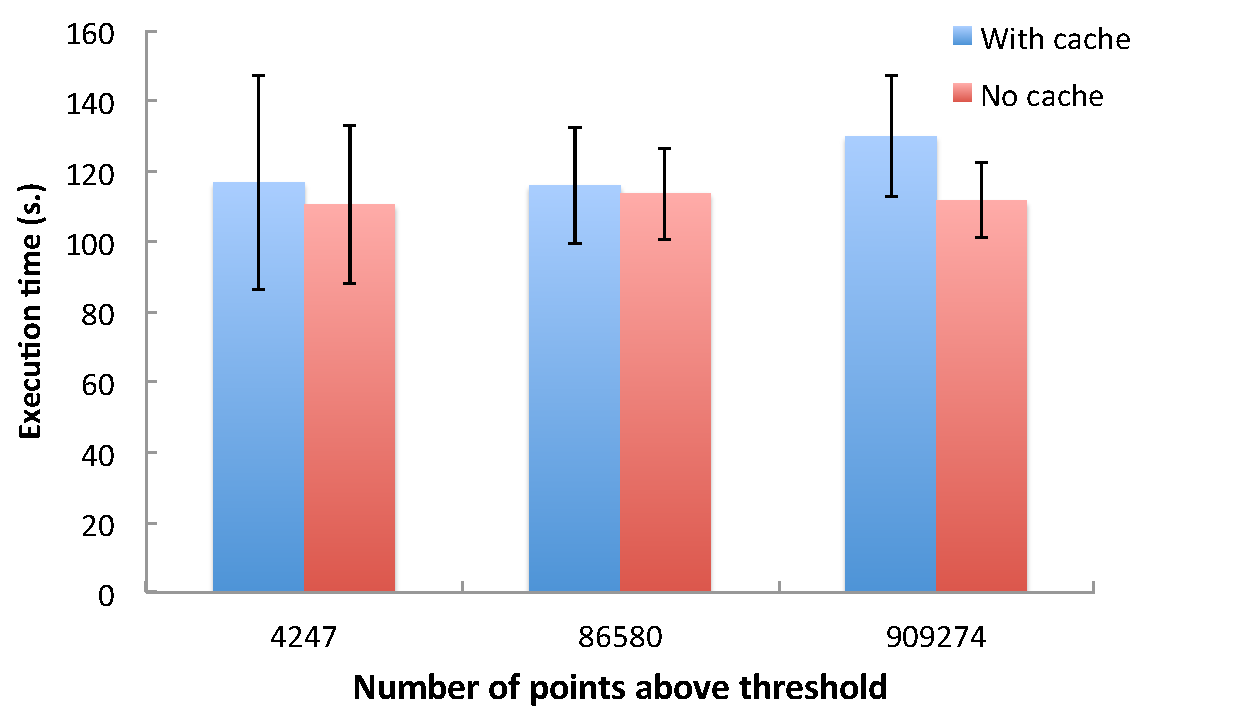
\includegraphics[width=3.35in]{Figures/cache_overhead.pdf}
\caption{Execution time for threshold queries at different threshold levels compared with the execution time of the same queries in the absence of a cache.}
\label{fig:cache_overhead}
\end{figure}

{\bf Overall execution of threshold queries}. The overall execution of threshold queries to the JHTDB is the following. The mediator submits a query to each of the database nodes storing the raw data
asynchronously. Each node begins evaluation of the query by first performing a cache lookup. If the data for the requested field, time-step and spatial region
are available in the cache and if the specified threshold is higher than the one stored in the cache the query can be answered from there. The records are
retrieved from the cache and the ones that have a higher value are returned to the mediator and subsequently back to the user. If the data stored in the
cache have a higher threshold than the one requested the cache needs to be updated. Similarly, if the cache does not have an entry for the specified 
parameters the query needs to be evaluated from the raw data. In those cases the raw data are read into memory with data along the boundary requested from
adjacent nodes as needed. The specified field is derived at each location on the grid and the norm or absolute value of the field is compared against
the threshold. The locations where the values are higher than the threshold need to then be stored in the cache. If the cache does not have enough space
for the new records, space is freed up by removing the least recently used data.  Reading from, updating or modifying the cache is done within a
transaction with snapshot isolation level. Snapshot isolation allows us to avoid locking the tables that serve as the cache for each transaction. This
provides for a higher degree of parallelism and avoids any potential deadlocks from queries running in parallel. Figure \ref{fig:cache_diagram} illustrates 
this process.

\section{Experimental Results}
We evaluate the developed method for the execution of threshold queries to large numerical simulation datasets with the goal of analyzing the 
benefits and overhead from the introduction of the application-aware cache. We also analyze the scaling properties of the method. Finally, we show
that an integrated method that performs the evaluation on the database nodes near the data is several orders of magnitude faster than evaluating
a threshold locally by the user.

\begin{figure}
\centering
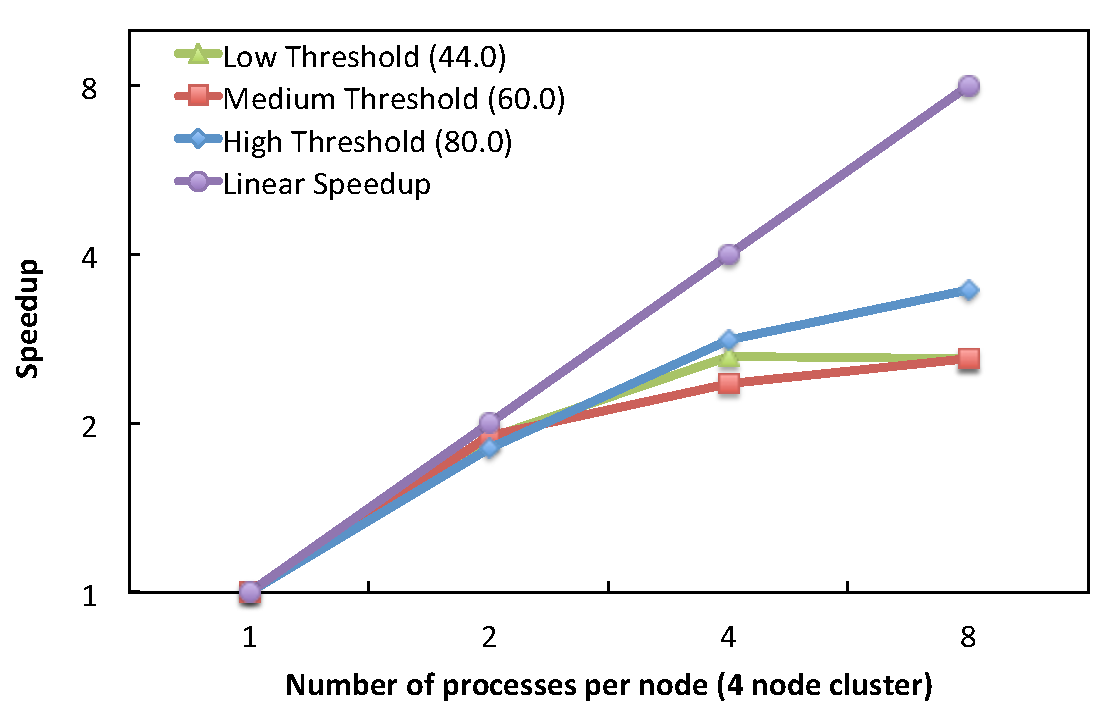
\includegraphics[width=3.35in]{Figures/scaleup.pdf}
\caption{Execution time for threshold queries at different threshold levels -- high, medium and low. The evaluation was performed utilizing 1-8
threads per server showcasing the vertical scalability of the implementation.}
\label{fig:scaleup}
\end{figure}

\subsection{Experimental Setup}
The experiments were run on the production database nodes of the JHTDB through a development Web-server hosting the Web-services. We used
the MHD dataset for the experimental runs. This dataset is partitioned across 4 database nodes according to spatial regions in the Morton z-order. 
The database nodes are 2.66 GHz dual quad-core Windows 2008 servers with SQL Server 2008 R2 and 24 GB of memory. Each node has 24 2TB 
SATA disks arranged as a set of four RAID-5 arrays. The database files are distributed in a round-robin fashion across the nodes and their associated disk
arrays. The tables storing the data are partitioned spatially along contiguous ranges of the Morton z-curve and the data for each partition reside in one
database file. 

For this evaluation we looked at the performance of threshold queries to the vorticity field. The vorticity field is representative of derived fields, which
have to be computed from the stored data. It defined as the curl of the velocity field.
As described in section \ref{science_use_cases}
thresholding the vorticity field is important in the study of fluid dynamics and obtaining the locations of maximum vorticity can lead to new insights into
the development of the most intense vortices that are observed. 
%\kk{Consider showing other fields as well; possibly thresholding the velocity by itself}

\subsection{Evaluation of cache effectiveness}

The central part of the strategy that we have developed for the evaluation of threshold queries of derived fields is the application-aware cache, which
stores the results of these queries. We first evaluate the overhead associated with the introduction and maintenance of the cache. Fig. \ref{fig:cache_overhead}
compares the execution time of queries in the absence of a cache with the execution time of the same queries, which interrogate the cache first.
For these experiments we requested
the locations with norms of the vorticity above thresholds at different levels. We refer the reader to Fig. \ref{fig:pdf}, which shows the distribution of values of
the norm of the vorticity field in the MHD dataset to get an appreciation of the different threshold values used in the experiments. 
For the first set the threshold was set high (80.0) and only $\sim$4,300 points 
(or 0.0004\% of all points) were above the threshold. For the second set a medium threshold (60.0) was chosen and $\sim$87,000 points 
(or 0.0081\% of all points) were above the threshold. Finally, a low threshold (44.0) was chosen for the last set with $\sim$900,000 points 
(or 0.0847\% of all points) above the threshold. For each set a random
time-step was chosen and the queries were run against that time-step. The measurements were taken from the point of view of the end user. 

The cache was initially populated by executing several hundred unrelated queries and contained several million entries.
Cache entries for the particular time-step queried were dropped before each run, making sure that each query would produce a cache miss and would
have to be evaluated from the raw data. 
The execution times were averaged over 10 runs.
We utilized 4 threads per database
node for the evaluation of each query. As we can see from the results the overhead associated with querying the cache first is minimal, 
less than 3\% and within
the margin of error. Additionally, the method shows stable running time across different time-steps and threshold levels. The slight increase in the running
time that can be observed is due to the larger result set that has to be returned to the user.

\begin{figure}
\centering
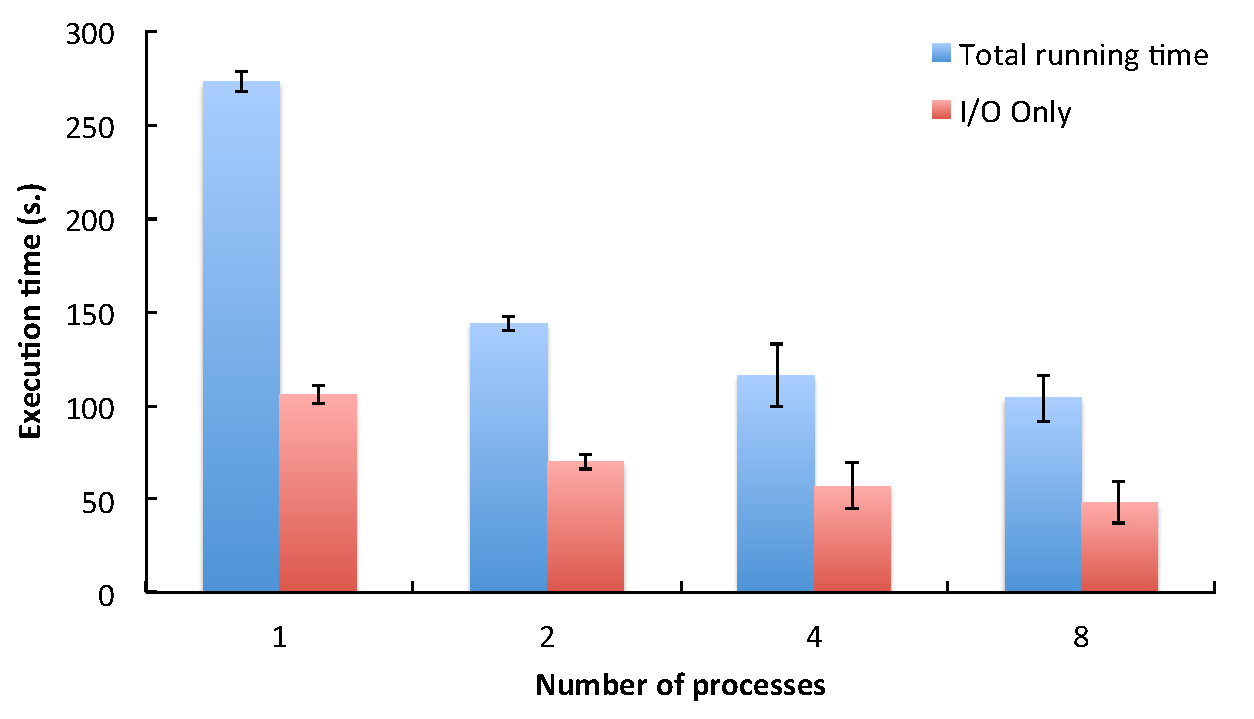
\includegraphics[width=3.35in]{Figures/io_comparison.pdf}
\caption{Execution time for threshold queries evaluated utilizing different number of
threads per server compared with the time taken to perform the I/O only.}
\label{fig:io_comparison}
\end{figure}

\begin{table}[h]
\centering
\begin{tabular}{|c|c|c|c|c|} \hline
\multirow{2}{0.5in}{Threshold} & \multirow{2}{0.5in}{Points above threshold} & \multicolumn{3}{|c|}{Running time (s.)}\\ \cline{3-5}
& & No cache & \parbox[t]{0.55in}{With cache (miss)} & \parbox[t]{0.55in}{With cache (hit)} \\ \hline
80.0 & 4247 & 97.1 & 100.2 & 0.5\\ \hline
60.0 & 86580 & 113.7 & 115.9 & 1.2\\ \hline
44.0 & 909274 & 111.6 & 115.0 & 9.1\\ \hline
\end{tabular}
\caption{Effectiveness of caching.}
\label{tab:cache_effectiveness}
\end{table}

Table \ref{tab:cache_effectiveness} shows the effectiveness of the cache in the case of a cache hit. It includes the data from Fig. \ref{fig:cache_overhead}
for the cases of execution in the absence of a cache and for cache misses. In the last column we show the running time of queries for which there is a 
cache hit. To simulate this scenario we first warm up the cache by submitting the same set of threshold queries of the vorticity field as before. We then submit
several more unrelated queries with different time-steps and threshold values in order to pollute the cache. Finally, we issue the original set of queries and 
measure their running times. As we can see from these results the introduction of an application-aware cache for the results of threshold queries yields over
an order of magnitude improvement for queries that hit the cache even for queries that have a low threshold and large result sets. Let us focus on the query
with low threshold, which returns $\sim$900,000 points. Given that the number of points that can be returned from a threshold query is limited to 1,000,000
it is likely that all subsequent queries to this time-step will result in a cache hit as their threshold is likely to be equal or higher than the cached one.

\subsection{Scaling and Distributed Evaluation}
The data-parallel evaluation of threshold queries exhibits good vertical scaling as shown in Fig. \ref{fig:scaleup}. For these experiments we used the same
queries and threshold values as for the runs shown in Fig. \ref{fig:cache_overhead} and Table \ref{tab:cache_effectiveness} 
but with varying number of threads per node. Cache entries for the
time-step queried were again dropped before each run in order to evaluate the scaling properties of the computation of the derived field from the stored data.
The computations for all of 
the derived fields of interest (such as the vorticity) at each gird point need data from adjacent grid points only. Therefore, each node of the cluster is able to
compute the derived field from data available locally with only a little amount along the boundary of each region having to be retrieved from adjacent nodes.
Each computation is independent and can be executed in parallel. This allows us to make use of multiple threads per node. 

We observer nearly a two times speedup when going from a single thread per node to two threads per node. The speedup diminishes to 1.4 times when going 
to 4 threads and little speedup is 
observed with 8 threads per node. This is due to several factors. Each node has 2 CPUs and a total of 8 cores, which need to run operating system and other SQL Server
processes as well. The experiments were run on the live production database nodes, which were also servicing other user queries. Additionally, SQL
Server already utilizes parallelism to perform most of the I/O. Finally, due to the data-parallel approach to the evaluation of these queries the data atoms along
the boundary of each region will be requested by multiple threads. Nevertheless, running with 4 threads per node is nearly 2.6 times faster when compared to
running a single thread.
\kk{Should we have scale-out experiments as well?}

Fig. \ref{fig:io_comparison} compares the running time of the queries with a medium threshold and executed with varying number of threads per node with
the time taken to perform the I/O only. The I/O time is about half of the total running time for these queries. As expected weaker than linear scale-up is 
observed for the I/O when additional threads are utilized. SQL Server already makes use of parallelism internally and the data have to be retrieved from the
same set of disks. It is worth noting that the total running time for the queries evaluated with 4 or 8 threads is about the same as the time it takes to perform the
I/O only with a single thread.

-- compare with local evaluation

\section{Related Work}
The processing of top-$k$ queries has been studied extensively in the context of distributed and relational database systems. A survey of different techniques
in the case of centralized processing is given in \cite{Ilyas}. In the case of distributed processing different approaches focus on horizontally 
\cite{Balke, Vlachou} or vertically \cite{Cao, Chaudhuri, Guntzer, Marian, Michel} distributed data. None of these approaches deals with array data stored in
a realtional database system. Moreover, these approaches focus on top-$k$ queries that use simple linear score functions to aggregate the atribute values of
individual records. In addition to top-$k$ queries we are also interested in threshold queries, where the result set includes all locations and values that are
above a user prescribed threshold. 

Zhao et al. propose an algorithm for the processing of top-$k$ queries in large-scale distributed environments called BRANCA \cite{Zhao}. They build on the 
idea of semantic caching \cite{Ren} and make use of branch caches, which store results of previous top-$k$ queries with respect to the data stored on each server.
The caching mecahnism that we use is similar in that regard, but the queries that are evaluated in our system operate on derived fields, which are computed
at each location by accessing data from a surrounding region. The queries described in \cite{Zhao} operate over the attributes of individual records only using
simple linear score functions.

A{\ss}falg et al. introduce the concept of threshold queries in time series databases \cite{Asfalg}. Their definition of threshold queries differs from the threshold
queries described in this paper. They are concerned with determining the time series, which exceed a user-defined threshold at time frames similar to
the time series specified in the query. Thus, their definition of threshold queries is concerned with the temporal relationship between the time series
stored in the database (usually one dimensional sequence of measurements) and the time series given in the query. In contrast, our approach focuses on
reporting all of the spatial locations of a multidimensional field where the norm or absolute value of the field exceeds a user prescribed threshold.

In a system called the tree cache Lopez et al. \cite{Lopez} make use of a small application-aware cache to reduce access time to large datasets stored on
disk. The tree cache stores individual octants of octree datasets and exploits application-specific information to determine which octants to cache and to 
perform query reordering. This work has inspired the use of an application-aware cache for the evaluation of threshold queries. In contrast to the tree cache
we do not cache raw data objects, but rather query results. This substantially reduces the size of the cache and improves query performance.

\section{Conclusions and Future Work}

We have presented an efficient strategy for the evaluation of threshold queries of derived fields in large numerical simulation datasets. 
The fields, which are thresholded are derived from the stored simulation data in a distributed data-parallel manner. The computations
scale with the cluster resources and are performed on the database nodes, where the data are stored. This new capability allows researches to quickly
obtain and focus on regions of special interest even if they lack the computing capabilities or data transfer rates necessary to examine entire time-steps
or large parts of the entire dataset. 

We have introduced an application-aware cache for the query results. The cache adds minimal overhead during the evaluation of queries even if there is
a cache miss and has modest storage requirements. Cache hits reduce query running times by over an order of magnitude.

The introduction of an application-aware cache for query results lays the ground work for the creation of a landmark database. Such a database can store the 
locations of the highest vorticity regions in the dataset or more broadly regions of interest and their associated statistics.

The Web-services approach to archived numerical simulation datasets provides public access to high quality simulation data to anyone with an internet
connection. The Web-services methods can be called from any modern programming language and we provide C, Fortran and Matlab client libraries for the
JHTDB. The evaluation of each query submitted through a Web-service call is carried out on the nodes of the database cluster by mens of a stored procedure
or a user-defined function that has been implemented and deployed to handle these requests. This allows us to fine-tune the execution of these procedures
and handle all requests transparently to the user. However, this approach also has drawbacks. Adding new functionality means adding to a long list of 
Web-service calls and requires substantial implementation effort. In the case of threshold queries the stored procedure performing the evaluation must have
an implementation for each derived field of interest even though the execution is handled by the same Web-service call. 

In the future we plan to develop
declarative and graphical user interfaces that will allow users to combine existing building blocks and perform computations that have not been explicitly
implemented. Additionally, we plan on deploying a server-side computing environment for users similar to the CasJobs service for the Sloan Digital Sky Survery \cite{LiThakar}. In such an environment users can run queries in batch mode and save their results in a personal database called MyDB, which 
will allow for much greater flexibility in the type of computations that can be performed in addition to substantially decreasing the network overhead.

%% \section{The {\secit Body} of The Paper}
%% Typically, the body of a paper is organized
%% into a hierarchical structure, with numbered or unnumbered
%% headings for sections, subsections, sub-subsections, and even
%% smaller sections.  The command \texttt{{\char'134}section} that
%% precedes this paragraph is part of such a
%% hierarchy.\footnote{This is the second footnote.  It
%% starts a series of three footnotes that add nothing
%% informational, but just give an idea of how footnotes work
%% and look. It is a wordy one, just so you see
%% how a longish one plays out.} \LaTeX\ handles the numbering
%% and placement of these headings for you, when you use
%% the appropriate heading commands around the titles
%% of the headings.  If you want a sub-subsection or
%% smaller part to be unnumbered in your output, simply append an
%% asterisk to the command name.  Examples of both
%% numbered and unnumbered headings will appear throughout the
%% balance of this sample document.

%% Because the entire article is contained in
%% the \textbf{document} environment, you can indicate the
%% start of a new paragraph with a blank line in your
%% input file; that is why this sentence forms a separate paragraph.

%% \subsection{Type Changes and {\subsecit Special} Characters}
%% We have already seen several typeface changes in this sample.  You
%% can indicate italicized words or phrases in your text with
%% the command \texttt{{\char'134}textit}; emboldening with the
%% command \texttt{{\char'134}textbf}
%% and typewriter-style (for instance, for computer code) with
%% \texttt{{\char'134}texttt}.  But remember, you do not
%% have to indicate typestyle changes when such changes are
%% part of the \textit{structural} elements of your
%% article; for instance, the heading of this subsection will
%% be in a sans serif\footnote{A third footnote, here.
%% Let's make this a rather short one to
%% see how it looks.} typeface, but that is handled by the
%% document class file. Take care with the use
%% of\footnote{A fourth, and last, footnote.}
%% the curly braces in typeface changes; they mark
%% the beginning and end of
%% the text that is to be in the different typeface.

%% You can use whatever symbols, accented characters, or
%% non-English characters you need anywhere in your document;
%% you can find a complete list of what is
%% available in the \textit{\LaTeX\
%% User's Guide}\cite{Lamport:LaTeX}.

%% \subsection{Math Equations}
%% You may want to display math equations in three distinct styles:
%% inline, numbered or non-numbered display.  Each of
%% the three are discussed in the next sections.

%% \subsubsection{Inline (In-text) Equations}
%% A formula that appears in the running text is called an
%% inline or in-text formula.  It is produced by the
%% \textbf{math} environment, which can be
%% invoked with the usual \texttt{{\char'134}begin. . .{\char'134}end}
%% construction or with the short form \texttt{\$. . .\$}. You
%% can use any of the symbols and structures,
%% from $\alpha$ to $\omega$, available in
%% \LaTeX\cite{Lamport:LaTeX}; this section will simply show a
%% few examples of in-text equations in context. Notice how
%% this equation: \begin{math}\lim_{n\rightarrow \infty}x=0\end{math},
%% set here in in-line math style, looks slightly different when
%% set in display style.  (See next section).

%% \subsubsection{Display Equations}
%% A numbered display equation -- one set off by vertical space
%% from the text and centered horizontally -- is produced
%% by the \textbf{equation} environment. An unnumbered display
%% equation is produced by the \textbf{displaymath} environment.

%% Again, in either environment, you can use any of the symbols
%% and structures available in \LaTeX; this section will just
%% give a couple of examples of display equations in context.
%% First, consider the equation, shown as an inline equation above:
%% \begin{equation}\lim_{n\rightarrow \infty}x=0\end{equation}
%% Notice how it is formatted somewhat differently in
%% the \textbf{displaymath}
%% environment.  Now, we'll enter an unnumbered equation:
%% \begin{displaymath}\sum_{i=0}^{\infty} x + 1\end{displaymath}
%% and follow it with another numbered equation:
%% \begin{equation}\sum_{i=0}^{\infty}x_i=\int_{0}^{\pi+2} f\end{equation}
%% just to demonstrate \LaTeX's able handling of numbering.

%% \subsection{Citations}
%% Citations to articles \cite{bowman:reasoning, clark:pct, braams:babel, herlihy:methodology},
%% conference
%% proceedings \cite{clark:pct} or books \cite{salas:calculus, Lamport:LaTeX} listed
%% in the Bibliography section of your
%% article will occur throughout the text of your article.
%% You should use BibTeX to automatically produce this bibliography;
%% you simply need to insert one of several citation commands with
%% a key of the item cited in the proper location in
%% the \texttt{.tex} file \cite{Lamport:LaTeX}.
%% The key is a short reference you invent to uniquely
%% identify each work; in this sample document, the key is
%% the first author's surname and a
%% word from the title.  This identifying key is included
%% with each item in the \texttt{.bib} file for your article.

%% The details of the construction of the \texttt{.bib} file
%% are beyond the scope of this sample document, but more
%% information can be found in the \textit{Author's Guide},
%% and exhaustive details in the \textit{\LaTeX\ User's
%% Guide}\cite{Lamport:LaTeX}.

%% This article shows only the plainest form
%% of the citation command, using \texttt{{\char'134}cite}.
%% This is what is stipulated in the SIGS style specifications.
%% No other citation format is endorsed.

%% \subsection{Tables}
%% Because tables cannot be split across pages, the best
%% placement for them is typically the top of the page
%% nearest their initial cite.  To
%% ensure this proper ``floating'' placement of tables, use the
%% environment \textbf{table} to enclose the table's contents and
%% the table caption.  The contents of the table itself must go
%% in the \textbf{tabular} environment, to
%% be aligned properly in rows and columns, with the desired
%% horizontal and vertical rules.  Again, detailed instructions
%% on \textbf{tabular} material
%% is found in the \textit{\LaTeX\ User's Guide}.

%% Immediately following this sentence is the point at which
%% Table 1 is included in the input file; compare the
%% placement of the table here with the table in the printed
%% dvi output of this document.

%% \begin{table}
%% \centering
%% \caption{Frequency of Special Characters}
%% \begin{tabular}{|c|c|l|} \hline
%% Non-English or Math&Frequency&Comments\\ \hline
%% \O & 1 in 1,000& For Swedish names\\ \hline
%% $\pi$ & 1 in 5& Common in math\\ \hline
%% \$ & 4 in 5 & Used in business\\ \hline
%% $\Psi^2_1$ & 1 in 40,000& Unexplained usage\\
%% \hline\end{tabular}
%% \end{table}

%% To set a wider table, which takes up the whole width of
%% the page's live area, use the environment
%% \textbf{table*} to enclose the table's contents and
%% the table caption.  As with a single-column table, this wide
%% table will ``float" to a location deemed more desirable.
%% Immediately following this sentence is the point at which
%% Table 2 is included in the input file; again, it is
%% instructive to compare the placement of the
%% table here with the table in the printed dvi
%% output of this document.

%% \begin{table*}
%% \centering
%% \caption{Some Typical Commands}
%% \begin{tabular}{|c|c|l|} \hline
%% Command&A Number&Comments\\ \hline
%% \texttt{{\char'134}alignauthor} & 100& Author alignment\\ \hline
%% \texttt{{\char'134}numberofauthors}& 200& Author enumeration\\ \hline
%% \texttt{{\char'134}table}& 300 & For tables\\ \hline
%% \texttt{{\char'134}table*}& 400& For wider tables\\ \hline\end{tabular}
%% \end{table*}
%% % end the environment with {table*}, NOTE not {table}!

%% \subsection{Figures}
%% Like tables, figures cannot be split across pages; the
%% best placement for them
%% is typically the top or the bottom of the page nearest
%% their initial cite.  To ensure this proper ``floating'' placement
%% of figures, use the environment
%% \textbf{figure} to enclose the figure and its caption.

%% This sample document contains examples of \textbf{.eps}
%% and \textbf{.ps} files to be displayable with \LaTeX.  More
%% details on each of these is found in the \textit{Author's Guide}.

%% \begin{figure}
%% \centering
%% \epsfig{file=fly.eps}
%% \caption{A sample black and white graphic (.eps format).}
%% \end{figure}

%% \begin{figure}
%% \centering
%% \epsfig{file=fly.eps, height=1in, width=1in}
%% \caption{A sample black and white graphic (.eps format)
%% that has been resized with the \texttt{epsfig} command.}
%% \end{figure}

%% As was the case with tables, you may want a figure
%% that spans two columns.  To do this, and still to
%% ensure proper ``floating'' placement of tables, use the environment
%% \textbf{figure*} to enclose the figure and its caption.

%% Note that either {\textbf{.ps}} or {\textbf{.eps}} formats are
%% used; use
%% the \texttt{{\char'134}epsfig} or \texttt{{\char'134}psfig}
%% commands as appropriate for the different file types.

%% \subsection{Theorem-like Constructs}
%% Other common constructs that may occur in your article are
%% the forms for logical constructs like theorems, axioms,
%% corollaries and proofs.  There are
%% two forms, one produced by the
%% command \texttt{{\char'134}newtheorem} and the
%% other by the command \texttt{{\char'134}newdef}; perhaps
%% the clearest and easiest way to distinguish them is
%% to compare the two in the output of this sample document:

%% This uses the \textbf{theorem} environment, created by
%% the\linebreak\texttt{{\char'134}newtheorem} command:
%% \newtheorem{theorem}{Theorem}
%% \begin{theorem}
%% Let $f$ be continuous on $[a,b]$.  If $G$ is
%% an antiderivative for $f$ on $[a,b]$, then
%% \begin{displaymath}\int^b_af(t)dt = G(b) - G(a).\end{displaymath}
%% \end{theorem}

%% The other uses the \textbf{definition} environment, created
%% by the \texttt{{\char'134}newdef} command:
%% \newdef{definition}{Definition}
%% \begin{definition}
%% If $z$ is irrational, then by $e^z$ we mean the
%% unique number which has
%% logarithm $z$: \begin{displaymath}{\log e^z = z}\end{displaymath}
%% \end{definition}

%% \begin{figure}
%% \centering
%% \psfig{file=rosette.ps, height=1in, width=1in,}
%% \caption{A sample black and white graphic (.ps format) that has
%% been resized with the \texttt{psfig} command.}
%% \end{figure}

%% Two lists of constructs that use one of these
%% forms is given in the
%% \textit{Author's  Guidelines}.

%% \begin{figure*}
%% \centering
%% \epsfig{file=flies.eps}
%% \caption{A sample black and white graphic (.eps format)
%% that needs to span two columns of text.}
%% \end{figure*}
%% and don't forget to end the environment with
%% {figure*}, not {figure}!
 
%% There is one other similar construct environment, which is
%% already set up
%% for you; i.e. you must \textit{not} use
%% a \texttt{{\char'134}newdef} command to
%% create it: the \textbf{proof} environment.  Here
%% is a example of its use:
%% \begin{proof}
%% Suppose on the contrary there exists a real number $L$ such that
%% \begin{displaymath}
%% \lim_{x\rightarrow\infty} \frac{f(x)}{g(x)} = L.
%% \end{displaymath}
%% Then
%% \begin{displaymath}
%% l=\lim_{x\rightarrow c} f(x)
%% = \lim_{x\rightarrow c}
%% \left[ g{x} \cdot \frac{f(x)}{g(x)} \right ]
%% = \lim_{x\rightarrow c} g(x) \cdot \lim_{x\rightarrow c}
%% \frac{f(x)}{g(x)} = 0\cdot L = 0,
%% \end{displaymath}
%% which contradicts our assumption that $l\neq 0$.
%% \end{proof}

%% Complete rules about using these environments and using the
%% two different creation commands are in the
%% \textit{Author's Guide}; please consult it for more
%% detailed instructions.  If you need to use another construct,
%% not listed therein, which you want to have the same
%% formatting as the Theorem
%% or the Definition\cite{salas:calculus} shown above,
%% use the \texttt{{\char'134}newtheorem} or the
%% \texttt{{\char'134}newdef} command,
%% respectively, to create it.

%% \subsection*{A {\secit Caveat} for the \TeX\ Expert}
%% Because you have just been given permission to
%% use the \texttt{{\char'134}newdef} command to create a
%% new form, you might think you can
%% use \TeX's \texttt{{\char'134}def} to create a
%% new command: \textit{Please refrain from doing this!}
%% Remember that your \LaTeX\ source code is primarily intended
%% to create camera-ready copy, but may be converted
%% to other forms -- e.g. HTML. If you inadvertently omit
%% some or all of the \texttt{{\char'134}def}s recompilation will
%% be, to say the least, problematic.

%% \section{Conclusions}
%% This paragraph will end the body of this sample document.
%% Remember that you might still have Acknowledgments or
%% Appendices; brief samples of these
%% follow.  There is still the Bibliography to deal with; and
%% we will make a disclaimer about that here: with the exception
%% of the reference to the \LaTeX\ book, the citations in
%% this paper are to articles which have nothing to
%% do with the present subject and are used as
%% examples only.
%% %\end{document}  % This is where a 'short' article might terminate

\section{Acknowledgment}

The authors would like to thank the Turbulence Database Group at Johns Hopkins University for
their insightful comments and suggestions. This work is supported in part by the National Science Foundation
under Grants ....

%% %ACKNOWLEDGMENTS are optional
%% \section{Acknowledgments}
%% This section is optional; it is a location for you
%% to acknowledge grants, funding, editing assistance and
%% what have you.  In the present case, for example, the
%% authors would like to thank Gerald Murray of ACM for
%% his help in codifying this \textit{Author's Guide}
%% and the \textbf{.cls} and \textbf{.tex} files that it describes.

%
% The following two commands are all you need in the
% initial runs of your .tex file to
% produce the bibliography for the citations in your paper.
\bibliographystyle{abbrv}
\bibliography{paper}  % sigproc.bib is the name of the Bibliography in this case
% You must have a proper ".bib" file
%  and remember to run:
% latex bibtex latex latex
% to resolve all references
%
% ACM needs 'a single self-contained file'!
%
%APPENDICES are optional
%\balancecolumns
%% \appendix
%% %Appendix A
%% \section{Headings in Appendices}
%% The rules about hierarchical headings discussed above for
%% the body of the article are different in the appendices.
%% In the \textbf{appendix} environment, the command
%% \textbf{section} is used to
%% indicate the start of each Appendix, with alphabetic order
%% designation (i.e. the first is A, the second B, etc.) and
%% a title (if you include one).  So, if you need
%% hierarchical structure
%% \textit{within} an Appendix, start with \textbf{subsection} as the
%% highest level. Here is an outline of the body of this
%% document in Appendix-appropriate form:
%% \subsection{Introduction}
%% \subsection{The Body of the Paper}
%% \subsubsection{Type Changes and  Special Characters}
%% \subsubsection{Math Equations}
%% \paragraph{Inline (In-text) Equations}
%% \paragraph{Display Equations}
%% \subsubsection{Citations}
%% \subsubsection{Tables}
%% \subsubsection{Figures}
%% \subsubsection{Theorem-like Constructs}
%% \subsubsection*{A Caveat for the \TeX\ Expert}
%% \subsection{Conclusions}
%% \subsection{Acknowledgments}
%% \subsection{Additional Authors}
%% This section is inserted by \LaTeX; you do not insert it.
%% You just add the names and information in the
%% \texttt{{\char'134}additionalauthors} command at the start
%% of the document.
%% \subsection{References}
%% Generated by bibtex from your ~.bib file.  Run latex,
%% then bibtex, then latex twice (to resolve references)
%% to create the ~.bbl file.  Insert that ~.bbl file into
%% the .tex source file and comment out
%% the command \texttt{{\char'134}thebibliography}.
%% % This next section command marks the start of
%% % Appendix B, and does not continue the present hierarchy
%% \section{More Help for the Hardy}
%% The acm\_proc\_article-sp document class file itself is chock-full of succinct
%% and helpful comments.  If you consider yourself a moderately
%% experienced to expert user of \LaTeX, you may find reading
%% it useful but please remember not to change it.
%% \balancecolumns
%% % That's all folks!
\end{document}
